\section{Third Member}
This is the section dedicated to one of the team members, and it should be written individually . It can include a range of things; first subsection is a space for you to point out the strengths and weaknesses of the module, including complaints about the module coordinator Max Wilson. The second section should have a selfie image with Max! The last part of it is the most important one. You will need to write a paragraph about what you have learned in this module. You can write it in \textbf{Bold} if you want or you can use other fonts. 

Please do not forget:
\begin{itemize}
	\item First paragraph should have your comments about the module
	\item Second one, a selfie img with Max
	\item Last one, what you learned in this module.
\end{itemize}

\subsection{Comments about the module}
The topic that is covered in the module is the most interesting so far. Before learning about all the different areas within FSE I wasn't sure what direction I was going to go career wise with my degree. The combination of computer science and communication with other people (not just solo coding) is brilliant.

The expected reading has been great. The book suggestion, even though it was slightly worded in a different ways, was also really helpful and gave me more understanding (in other ways). The lectures themselves were great too, there wasn't one that I felt rushed through time wise. The sheets handed out in the lectures didn't really do much for me. Generally very happy with the quality of them though compared to some other modules. Very clear, and explained well. The thing at the bottom of the slides showing where it relates in the subject is also a great idea.

\subsection{Selfie with Max}

To include an image, you will need to remove the comments from the code below, place an image in the main folder, and do not forget to put the name of the image instead of ImgName. 

\begin{figure}[h]
\caption{Selfie with Max}
\centering
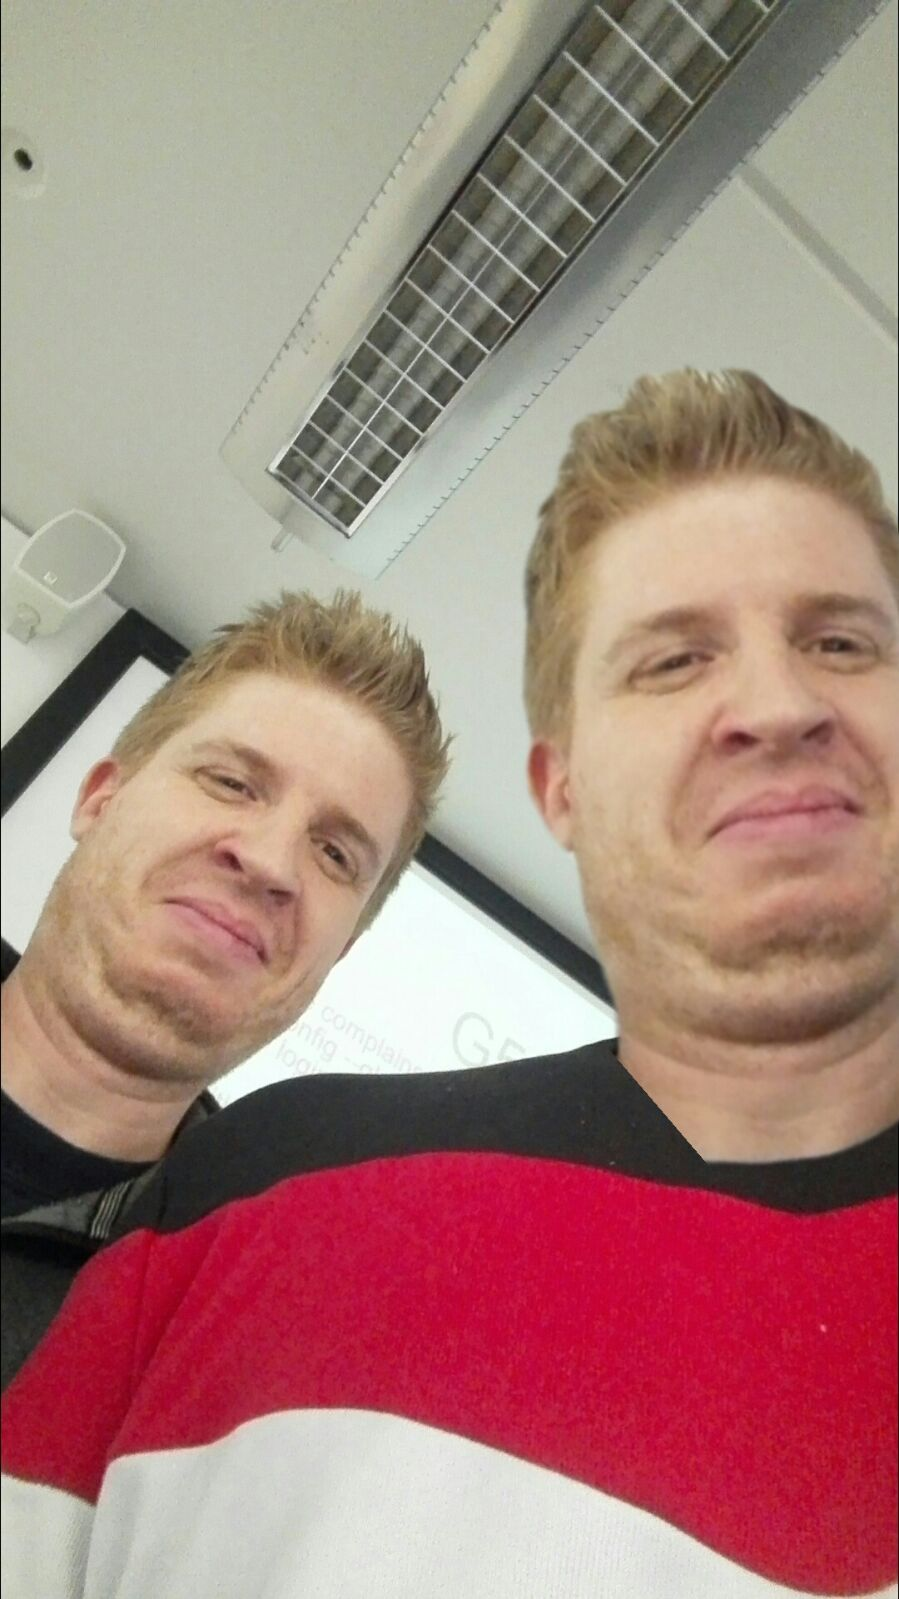
\includegraphics[width=0.5\textwidth]{af48bcf9-8756-467e-bd54-b3275c9d5df9.jpg}
\label{fig:selfie}
\end{figure}

You can then use the label of the figure to reference it later with the command ${\backslash}ref$. you can comment out the next line to see an example of how it works.

% My selfie with Max is in  Figure~\ref{fig:selfie}.

\subsection{What I have learned in this module}
There are so many layers to building software. It is not just staying up to 4am  code and getting it done. It requires planning and understanding as a group from beginning to end.

